% !TEX root = ../ausarbeitung.tex
%Erklärung des Nutzertests mit Testgruppe, was herausgefunden werden soll:
%A: Macht so ein Spiel für Partnerzahlen Spaß?
%B: Welche Version ist besser?
\chapter{Evaluation} %TODO Ref
Im Rahmen dieser Arbeit wurde versucht über den GEQ zwei Fragen zu beantworten. Zunächst sollte überprüft werden ob dieses Additionsspiel zur Unterstützung des Lernprozesses bei Addition über Partnerzahlen den Kindern Spaß bereitet. Außerdem sollte ermittelt werden welche der beiden implementierten Versionen besser bei den Kindern ankommt. Zur Beantwortung wurde der GEQ Fragebogen abgewandelt zur KidsGEQ Variante damit Grundschüler alle Fragen verstehen und beantworten können.
\section{Game Experience Questionnaire}
Beim normalen GEQ werden 3 Module eingebaut:
\begin{itemize}
\item Core questionaire
\item Social Presence Module
\item Post-game Module
\end{itemize}
Diese Module werden direkt nach einer Spielrunde durchgegangen, dabei testen die ersten beiden Module wie der Spieler sich beim spielen gefühlt hat, während das Post-Game Module testet wie der Spieler sich nach dem beenden des spielens gefühlt hat.
\subsection{Core questionaire}
In diesem Teil werden dem Spieler Fragen aus den Kategorien Challenge, Competence, Flow, Immersion, Negative Effect, Positive Effect und Tension gestellt. Um eine gute Messung zu erzielen und Puffer zu haben um wenn nötig Fragen streichen zu können, sollte man 5 Fragen pro Kategorie verwenden. In der Auswertung sollte hier außerdem die Gewichtung der Fragen überprüft werden, da es sein kann das bei der Ausführung mit einer Frage Probleme auftreten können. Wenn sie zum Beispiel nicht verstanden wurde, kann es sein das man diese Frage aus der Auswertung entfernen muss.
\subsubsection{Challenge}
Mit den Challenge Fragen wird beim GEQ der Schwierigkeitsgrad des Spiels ermittelt. Der Schwierigkeitsgrad des Spiels kann durch mehrere Faktoren beeinflusst werden. Zum einen kann die Aufgabe einfach schwer gewählt sein, aber auch durch die technische Umsetzung und dem Design kann der Schwierigkeitsgrad angehoben werden. Auf diesen Einfluss wird in der Diskussion noch weiter eingegangen.
\subsubsection{Competence}
In der Competence Kategorie sollen Fragen beantwortet werden, die darauf abzielen ob das Spiel intuitiv ist. Das heißt der Spieler sollte zu jeder Zeit wissen, was seine Aufgabe ist und wie er der Erfüllung dieses Ziels näher kommt.
\subsubsection{Flow}
Der Flow-Wert beschreibt wie stark das Spiel die Aufmerksamkeit des Spielers eingenommen hat und wie 'vertieft'  er in das Spiel war.
\subsubsection{Immersion}
In dieser Kategorie soll geprüft werden, wie die Ästhetik des Spiels ist. Dies betrifft sowohl ob das Spiel Visuell überzeugen konnte, als auch ob man durch das Spiel die Fantasie des Spielers anregen konnte.
\subsubsection{Negative Effect}
Hier soll über Fragen ermittelt werden, ob das Spiel negative Einflüsse auf den Spieler hat. Diese Einflüsse können dazu führen, dass das Spiel dem Spieler keinen Spaß bereitet. Bei bestimmten Genres, wie Horrorspielen, können negative Einflüsse, wie Angst, allerdings auch gewollt sein. Im Fall von MathSnake sollten diese aber möglichst minimiert werden.
\subsubsection{Positive Effect}
Unter dieser Kategorie versteht man Fragen, die ermitteln sollen ob das Spiel positive Einflüsse auf den Spieler hatte. Diese führen dazu, dass sich der Spieler durch das Spiel besser fühlt, da er zum Beispiel lachen musste.
\subsubsection{Tension}
In dieser Kategorie zielen die Fragen auf die Gemütslage des Spielers ab. Hier können Erkenntnisse darüber gewonnen werden ob das Spiel noch zu unausgereift ist. Dies ist dann der Fall, wenn der Spieler sich über das Spiel mehrfach beschwert, da er weiß wie er sein Ziel erreichen kann, aber zum Beispiel die Steuerung ist zu sensibel oder verzögert.
\subsubsection{Bestimmung der Kategoriewerte}
Um den Wert jeder Kategorie für einen Teilnehmer des Nutzertests zu bestimmen, werden die Antwortmöglichkeiten von 0 bis 4 gewichtet. Anschließend addiert man nach dieser Skala alle Werte der jeweiligen Kategorie auf und teilt ihn durch die Anzahl an Fragen. 
\subsection{Social Presence Module} %TODO Ref!
Das Social Presence Module wird benötigt um die psychologische und verhaltensbezogene Einbindung des Spielers ins Spielgeschehen zu messen. Dies geschieht entweder virtuel, durch In-Game Characteren mit denen Gesprochen werden kann so genannten NPC's, mediated, wenn das Spiel einen Online-Modus besitzt, oder co-located. Das Modul sollte nur dann eingesetzt werden, wenn mindestends eines dieser Einbindungen des Spielers vorhanden sind.
\subsection{Post-Game Module}
Das Post-Game Module wird verwendet um zu prüfen wie sich die Spieler nach dem Ende der Spielphase fühlen. Dieses Modul ist besonders deswegen relevant, da man hier ermitteln kann ob der Spieler zum Beispiel freiwillig spielen möchte oder eigentlich keine Lust mehr auf das Spiel hat.
\section{Umsetzung des KidsGEQ}
In der umgesetzten Version wurden pro Kategorie 3 Aussagen gewählt, die zunächst ins deutsche übersetzt wurden und anschließend in möglichst leicht für Kinder verständliche Sprache umformuliert. Diese 21 Aussagen sollen nun von den Kindern anhand einer Skala beantwortet werden. Diese Skala ist in 5 Kategorien aufgebaut: 'überhaupt nicht', 'ein wenig', 'mittel', 'ziemlich', 'sehr'. Die Frage an die Kinder ist wie stark sie der jeweiligen Aussage zustimmen. Der Grad der Zustimmung wird zusätzlich durch einen Farbcode hervorgehoben. 

\begin{figure}[htb]
	\centering
	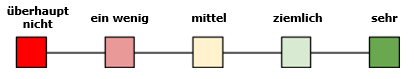
\includegraphics[width=0.75\textwidth]{farbskala}
	\caption{Farbskala der einzelnen Fragen\label{fig:farbskala}}
\end{figure}

Außerdem wurde eine weitere Frage mit dieser Skala hinzugefügt um abzufragen wie gut die Kinder mit der Steuerung zurecht gekommen sind. Abschließend zu diesen 22 Ankreuzfragen gab es noch 3 schriftliche Fragen um am Ende eine klare Antwort auf die Forschungsfragen zu forcieren. %TODO richtig mit forciert?
\section{Durchführung des Nutzertests} %TODO Zufällige Version?
Der Nutzertest wurde in 2 Phasen durchgeführt. Zunächst durften die Kinder eine Version für 10 Minuten spielen. Anschließend gab es den ersten Fragebogen mit den 22 Fragen. Nach einer kurzen Pause von ca. 5 Minuten in denen sich mit etwas komplett anderem beschäftigt wurde, ging es zu den zweiten 10 Minuten spielen der anderen Version. Nach dieser Spielzeit wurde wieder der Fragebogen ausgefüllt mit den abschließenden 3 schriftlichen Fragen. Insgesamt ergab dies eine Versuchsdauer von ca. 30 Minuten pro Person.\\
\\
Der Nutzertest wurde mit einer kleinen Anzahl an Kindern durchgeführt aufgrund dessen, dass in der Weihnachtszeit nur sehr schwer Testpersonen im Alter der Zielgruppe gefunden werden kann. Die Menge an Testpersonen umfasste 5 Grundschulkinder aus den ersten Klassenstufen. Diese kleine Menge lässt zwar keine statistischen Erhebungen zu, allerdings können wir darauf deskriptive Statistik anwenden. 

\hfil\rule{0.4\textwidth}{0.4pt}